\documentclass[a4paper,12pt]{article}

\usepackage[utf8]{inputenc}
\usepackage[left=0.5in,right=0.5in,top=1in,bottom=1in]{geometry}
\usepackage{amsmath,amssymb,amsfonts}
\usepackage{pgfplots,graphicx,calc,changepage}
\pgfplotsset{compat=newest}
\usepackage{enumitem}
\usepackage{fancyhdr}
\usepackage[colorlinks = true, linkcolor = blue]{hyperref}

% Syntax highlighting
\usepackage{listings}
\usepackage{xcolor}

\definecolor{codegreen}{rgb}{0.40,0.62,0.07}
\definecolor{codegray}{rgb}{0.5,0.5,0.5}
\definecolor{codeblue}{rgb}{0.09,0.57,0.73}
\definecolor{backcolour}{rgb}{1,1,1}

\lstdefinestyle{mystyle}{
    backgroundcolor=\color{backcolour},   
    commentstyle=\color{codegreen},
    keywordstyle=\color{magenta},
    numberstyle=\tiny\color{codegray},
    stringstyle=\color{codeblue},
    basicstyle=\ttfamily\small,
    breaklines=true,                     
    keepspaces=true,                 
    numbers=left,                    
    numbersep=5pt,                  
    showspaces=false,
    showstringspaces=false,
    showtabs=false,                  
    tabsize=4
}

\lstset{style=mystyle}

\newcommand{\bigO}{\mathcal{O}}
\newcommand{\nats}{\mathbb{N}}
\newcommand{\reals}{\mathbb{R}}
\newcommand{\rats}{\mathbb{Q}}
\newcommand{\ints}{\mathbb{Z}}
\newcommand{\comps}{\mathbb{C}}
\newcommand{\pols}{\mathcal{P}}
\newcommand{\cants}{\Delta\!\!\!\!\Delta}
\newcommand{\eps}{\varepsilon}
\newcommand{\st}{\backepsilon}
\newcommand{\abs}[1]{\left| #1 \right|}
\newcommand{\dom}[1]{\mathrm{dom}\left(#1\right)}
\newcommand{\for}{\text{ for }}
\newcommand{\dd}{\mathrm{d}}
\newcommand{\spn}{\mathrm{sp}}
\newcommand{\nul}{\mathcal{N}}
\newcommand{\col}{\mathrm{col}}
\newcommand{\rank}{\mathrm{rank}}
\newcommand{\norm}[1]{\lVert #1 \rVert}
\newcommand{\inner}[1]{\left\langle #1 \right\rangle}
\newcommand{\pmat}[1]{\begin{pmatrix} #1 \end{pmatrix}}
\renewcommand{\and}{\text{ and }}

\newsavebox{\qed}
\newenvironment{proof}[2][$\square$]
    {\setlength{\parskip}{0pt}\par\textit{Proof:} #2\setlength{\parskip}{0.25cm}
        \savebox{\qed}{#1}
        \begin{adjustwidth}{\widthof{Proof:}}{}
    }
    {
        \hfill\usebox{\qed}\end{adjustwidth}
    }

\pagestyle{fancy}
\fancyhead{}
\lhead{Caleb Jacobs}
\chead{APPM 5610: Numerical Analysis II}
\rhead{Homework \#7}
\cfoot{}
\setlength{\headheight}{35pt}
\setlength{\parskip}{0.25cm}
\setlength{\parindent}{0pt}

\begin{document}
\section{Problems}
\begin{enumerate}[label = (\arabic*)]
	\item Determine the order and the region of absolute stability of the s-step Adams-Bashforth methods for $ s = 2, 3 $,
	\[
		\begin{array}{crcl}
			s = 2: & y_{n + 2} & = & y_{n + 1} + h \left(\frac{3}{2} f(t_{n + 1}, y_{n + 1}) - \frac{1}{2}f(t_n, y_n)\right) \\
			s = 3: & y_{n + 3} & = & y_{n + 2} + h \left( \frac{23}{12} f(t_{n + 2}, y_{n + 2}) - \frac{4}{3} f(t_{n + 1}, y_{n + 1}) + \frac{5}{12} f(t_n, y_n) \right)
		\end{array}
	\]
	and the order and the region of absolute stability of the 2-step Adams-Moulton method,
	\[
		s = 2: y_{n + 2} = y_{n + 1} + h \left( \frac{5}{12} f(t_{n + 2}, y_{n + 2}) + \frac{2}{3} f(t_{n + 1}, y_{n + 1}) - \frac{1}{12}f(t_n, y_n) \right).
	\]
	\begin{center}
		\emph{My work begins on the next page.}
	\end{center}
	
	\newpage
	For the Adams-Bashforth method with $ s = 2 $, our order can be computed  the expansions given in the Appendix \ref{sec:app} and some simplification using Mathematica, the order can be computed as
	\begin{align*}
		y(t_{n + 2}) - y(t_{n + 1}) - h \left(\frac{3}{2} y'(t_{n + 1}) - \frac{1}{2} y'(t_n) \right) &= \frac{15}{12} h^3 y'''(t_n) + \bigO(h^4)
 	\end{align*}
	showing the order of this method is \emph{2}.
	
	Now, we can find the region of absolute stability by first computing the parametric boundary of the region as
	\begin{align*}
		\sum_{m = 0}^{2} a_m e^{i m \theta} &= -e^{i \theta} + e^{2 i \theta} = \underbrace{-\cos\theta +\cos 2\theta}_{A(\theta)} + i \underbrace{(-\sin \theta + \sin 2\theta)}_{B(\theta)} \\
		\sum_{m = 0}^{2} b_m e^{i m \theta} &= -\frac{1}{2} + \frac{3}{2} e^{i \theta} = \underbrace{-\frac{1}{2} + \frac{3}{2}\cos\theta}_{C(\theta)} + i \underbrace{\frac{3}{2}\sin\theta}_{D(\theta)}.
	\end{align*}

	Then, our parametric boundary is given by 
	\[
		r(\theta) = \frac{AC + BD}{C^2 + D^2} + i \frac{BC - AD}{C^2 + D^2}
	\]
	where, $ A, B, C, $ and $ D $ are given in the previous lines. Plotting this region in the complex plane yields
	
	\begin{figure}[h]
		\centering
		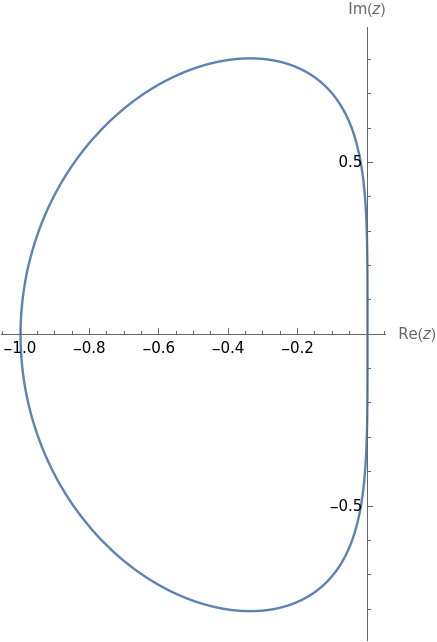
\includegraphics[width = 0.3 \textwidth]{Images/AB2.png}
	\end{figure}

	After checking a point inside of this boundary shows that our region of absolute stability is given by the region inside of this curve.
	
	\newpage
	Just as with $ s = 2 $, we can use the same expansions and some Mathematica simplification to get the order of the Adams-Bashforth method with $ s = 3 $ as
	\[
		y(t_{n + 3}) - y(t_{n + 2}) - h \left( \frac{23}{12} y'(t_{n + 2}) - \frac{4}{3} y'(t_{n + 1}) + \frac{5}{12} y'(t_n) \right) = \frac{3}{8} h^4 y^{(4)}(t_n) + \bigO(h^5)
	\]
	showing the order of this method is \emph{3}.
	
	Now, we can find the region of absolute stability by first computing the parametric boundary of the region as
	\begin{align*}
		\sum_{m = 0}^{3} a_m e^{i m \theta} &= -e^{2 i \theta} + e^{3 i \theta} = \underbrace{-\cos2\theta + \cos 3\theta}_{A(\theta)} + i \underbrace{(-\sin 2\theta + \sin 3\theta)}_{B(\theta)} \\
		\sum_{m = 0}^{3} b_m e^{i m \theta} &= \frac{5}{12} - \frac{4}{3} e^{i \theta} + \frac{23}{12} e^{2\theta} = \underbrace{\frac{5}{12} - \frac{4}{3} \cos \theta + \frac{23}{12} \cos 2\theta}_{C(\theta)} + i \underbrace{\left(-\frac{4}{3} \sin \theta + \frac{23}{12} \sin 2\theta\right)}_{D(\theta)}.
	\end{align*}

	Then, our parametric boundary is given by 
	\[
	r(\theta) = \frac{AC + BD}{C^2 + D^2} + i \frac{BC - AD}{C^2 + D^2}
	\]
	where, $ A, B, C, $ and $ D $ are given in the previous lines. Plotting this region in the complex plane yields
	
	\begin{figure}[h]
		\centering
		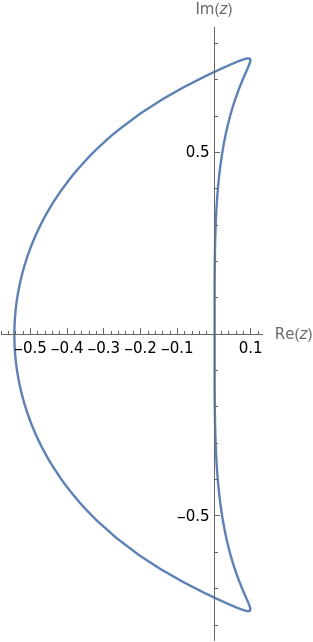
\includegraphics[width = 0.3 \textwidth]{Images/AB3.png}
	\end{figure}

	Similar to before, the stability of a point inside of this curve reveals that the region of absolute stability is given by the region inside of this curve.
	
	\newpage
	Finally, we can use the same strategy as before to compute 2-step Adams-Moulton method as
	\[
		y(t_{n +2}) - y(t_{n + 1}) - h \left( \frac{5}{12} y'(t_{n + 2}) + \frac{2}{3} y'(t_{n + 1}) - \frac{1}{12} y'(t_n) \right) = -\frac{1}{24} h^4 f^{(4)}(t_n) + \bigO(h^5)
	\]
	showing this method is order \emph{3}
	
	Now, we can find the region of absolute stability by first computing the parametric boundary of the region as
	\begin{align*}
		\sum_{m = 0}^{2} a_m e^{i m \theta} &= -e^{i \theta} + e^{2 i \theta} = \underbrace{-\cos\theta +\cos 2\theta}_{A(\theta)} + i \underbrace{(-\sin \theta + \sin 2\theta)}_{B(\theta)} \\
		\sum_{m = 0}^{2} b_m e^{i m \theta} &= -\frac{1}{12} + \frac{2}{3} e^{i \theta} + \frac{5}{12} e^{2i \theta} = \underbrace{-\frac{1}{12} + \frac{2}{3}\cos\theta + \frac{5}{12} \cos 2\theta}_{C(\theta)} + i \underbrace{\left(\frac{2}{3}\sin\theta + \frac{5}{12} \sin 2\theta\right)}_{D(\theta)}.
	\end{align*}
	
	Then, our parametric boundary is given by 
	\[
	r(\theta) = \frac{AC + BD}{C^2 + D^2} + i \frac{BC - AD}{C^2 + D^2}
	\]
	where, $ A, B, C, $ and $ D $ are given in the previous lines. Plotting this region in the complex plane yields
	
	\begin{figure}[h]
		\centering
		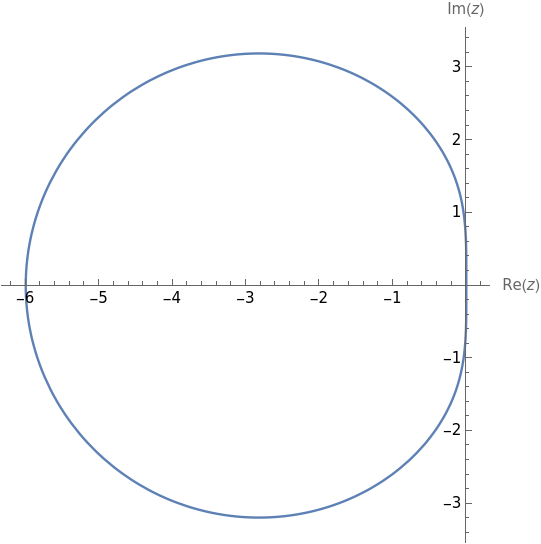
\includegraphics[width = 0.4 \textwidth]{Images/AM2.png}
	\end{figure}

	Just as before, checking the stability of a point inside of our curve shows that the region of absolute stability is given by the region inside of our curve.
	
	\newpage
	\item Determine the order and the region of absolute stability of BDF method of orders $ s = 2, 3 $:
	\[
		\begin{array}{crcl}
			s = 2: & y_{n + 2} - \frac{4}{3} y_{n + 1} + \frac{1}{3} y_n & = & \frac{2}{3} h f(x_{n + 2}, y_{n + 2}) \\
			s = 3: & y_{n + 3} - \frac{18}{11} y_{n + 2} + \frac{9}{11} y_{n + 1} - \frac{2}{11} y_n & = & \frac{6}{11} h f(x_{n + 3}, y_{n + 3}).
		\end{array}
	\]
	
	Just as in question 1, we can use the expansions in the Appendix \ref{sec:app} along with some simplifications from Mathematica to get the of the BDF formula with $ s = 2 $ as 
	\[
		y(t_{n + 2}) - \frac{4}{3} y(t_{n + 1}) + \frac{1}{3} y(t_n) - \frac{2}{3} h y'(t_{n + 2}) = -\frac{2}{9} h^3 y^{(3)}(t_n) + \bigO(h^4)
	\]
	showing this method is order \emph{2}.
	
	Just as in problem 1, we can find the region of absolute stability by first computing the parametric boundary of the region as
	\begin{align*}
		\sum_{m = 0}^{2} a_m e^{i m \theta} &= \frac{1}{3} - \frac{4}{3} e^{i \theta} + e^{2 i \theta} = \underbrace{\frac{1}{3} - \frac{4}{3} \cos\theta + \cos 2\theta}_{A(\theta)} + i \underbrace{\left(- \frac{4}{3} \sin\theta + \sin 2\theta\right)}_{B(\theta)} \\
		\sum_{m = 0}^{2} b_m e^{i m \theta} &= \frac{2}{3} e^{2i \theta} = \underbrace{\frac{2}{3} \cos 2\theta}_{C(\theta)} + i \underbrace{\frac{2}{3} \sin 2\theta}_{D(\theta)}.
	\end{align*}
	
	Then, our parametric boundary is given by 
	\[
	r(\theta) = \frac{AC + BD}{C^2 + D^2} + i \frac{BC - AD}{C^2 + D^2}
	\]
	where, $ A, B, C, $ and $ D $ are given in the previous lines. Plotting this region in the complex plane yields
	
	\begin{figure}[h]
		\centering
		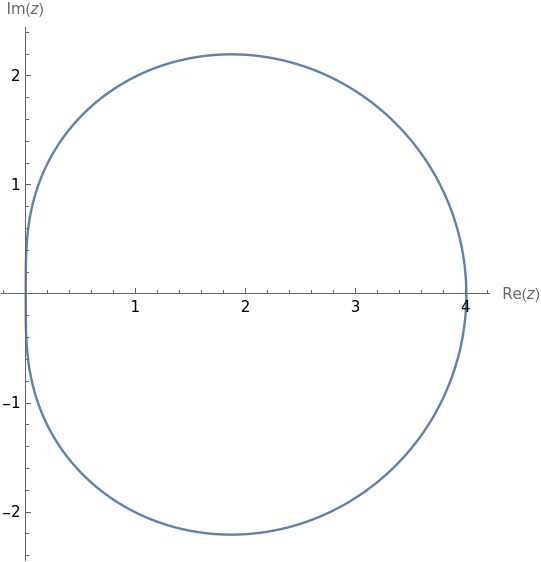
\includegraphics[width = 0.4 \textwidth]{Images/BDF2.png}
	\end{figure}

	Slightly different to problem 1, we check a point outside of this curve for stability. Doing so show that region of absolute stability is given by the region outside of the curve.
	
	\newpage
	Similarly, we can use the expansions in the Appendix \ref*{sec:app} to compute the order of the BDF formula with $ s = 3 $ as 
	\[
		y(t_{n + 3}) - \frac{18}{11} y(t_{n + 2}) + \frac{9}{11} y(t_{n + 1}) - \frac{2}{11} y(t_n) - \frac{6}{11} h y'(t_{n + 3}) = -\frac{3}{22} h^4 y^{(4)}(t_n) + \bigO(h^5)
	\]
	showing this method is order \emph{3}.
	
	Moving on, we can find the region of absolute stability by first computing the parametric boundary of the region as
	\begin{align*}
		\sum_{m = 0}^{3} a_m e^{i m \theta} = -\frac{2}{11} + \frac{9}{11} e^{i \theta} - \frac{18}{11} e^{2 i \theta} + e^{3 i \theta} =& \underbrace{-\frac{2}{11} + \frac{9}{11} \cos \theta - \frac{18}{11} \cos 2\theta + \cos 3\theta}_{A(\theta)} \\
		&+ i \underbrace{\left(\frac{9}{11} \cos \theta - \frac{18}{11} \cos 2\theta + \cos 3\theta\right)}_{B(\theta)} \\
		\sum_{m = 0}^{3} b_m e^{i m \theta} = \frac{6}{11} e^{3i \theta} = \underbrace{\frac{6}{11} \cos 3\theta}_{C(\theta)} + i \underbrace{\frac{6}{11} \sin 3\theta}_{D(\theta)}.
	\end{align*}
	
	Then, our parametric boundary is given by 
	\[
	r(\theta) = \frac{AC + BD}{C^2 + D^2} + i \frac{BC - AD}{C^2 + D^2}
	\]
	where, $ A, B, C, $ and $ D $ are given in the previous lines. Plotting this region in the complex plane yields
	
	\begin{figure}[h]
		\centering
		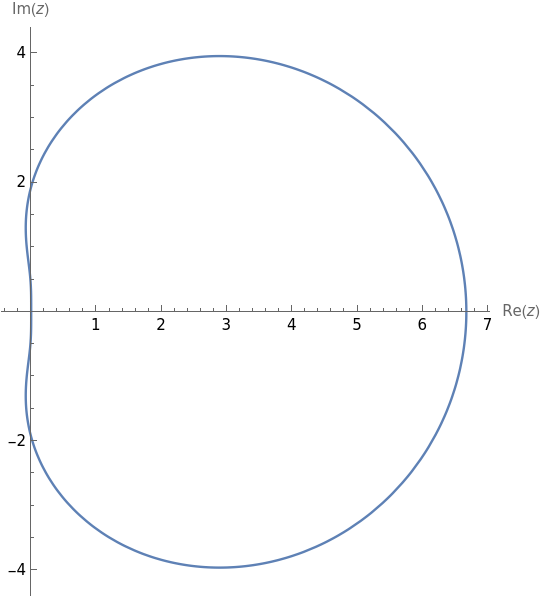
\includegraphics[width = 0.4 \textwidth]{Images/BDF3.png}
	\end{figure}

	Similar to the previous BDF formula, we check the stability at a point outside of our surface. Doing so yields a stable algorithm and so our region of absolute stability is given by the region outside of this curve.
\end{enumerate}

\newpage
\section{Appendix} \label{sec:app}
Taylor expansions used in order calculations:
\begin{align*}
	y(t_{n + 1}) &= y(t_n)+h y'(t_n)+\frac{1}{2} h^2 y''(t_n)+\frac{1}{6} h^3 y^{(3)}(t_n)+\frac{1}{24} h^4 y^{(4)}(t_n)+O\left(h^5\right) \\
	y(t_{n + 2}) & = y(t_n)+2 h y'(t_n)+2 h^2 y''(t_n)+\frac{4}{3} h^3 y^{(3)}(t_n)+\frac{2}{3} h^4 y^{(4)}(t_n)+O\left(h^5\right) \\
	y(t_{n + 3}) & = y(t_n)+3 h y'(t_n)+\frac{9}{2} h^2 y''(t_n)+\frac{9}{2} h^3 y^{(3)}(t_n)+\frac{27}{8} h^4 y^{(4)}(t_n)+O\left(h^5\right)
\end{align*}
\end{document}